\section{渲染的本质}
在渲染方面上的研究与优化已经发展成熟,已成为一个非常复杂的系统了,本文的目标是从理解渲染的技术原理,从软渲染,到CPU,再到GPU。
为简化,我们以图元三角形为例,主要有两个阶段:
\begin{itemize}
    \item {决定那些像素坐标构成这个三角形}
    \item {决定这些像素的颜色值是多少,这个过程就是着色shading}
\end{itemize}
它们分别对应着图形学中另外两个概念,光栅化和光照模型。

\subsection{光栅化Rasterize}

图形学中,是物理的三维世界,如何把三维物体在二维屏幕上显示,需要把它的三维属性都降为二维的结果,大致存在以下几个步骤:

\begin{itemize}
    \item {坐标变换}
    \item {属性计算,如颜色,纹理,alpha等}
    \item {光栅化}
\end{itemize}

目前大众屏幕分辨率为1920x1080,在二维屏幕渲染时,内存中的FrameBuffer只保存着1920x1080个屏幕点的颜色,然后再映射到屏幕上面。
光栅化的,就是计算出1920x1080个点的颜色值的过程。把物体的数学描述转换为屏幕的像素值,是从连续到离散,即物理的坐标是浮点数,而屏幕坐标是整数,光栅化的过程是一个近似的过程。
在一些图形处理软件中就是把矢量图形转化成像素点的过程。

\subsection{光照模型illumination model}
当光照射到物体表面时,物体会对光发生反射、透射、吸收、衍射、折射、干涉等。其中被物体吸收的部分转化为热。
反射、透射的光会进入人的视觉系统,使我们看见物体。为了模拟仿真这一真实的现象,建立一些数学模型来替代复杂的真实
物理模型,这些模型就称为光照模型。
\begin{itemize}
    \item {1971,Gourand提出,用漫反射模型计算多边形顶点的光亮度,再用增量法插值计算}
    \item {1975,Phong提出一个经验模型,真实度达到可以接受的程度}
    \item {1980,Whitted提出一个光透射模型,是第一个光线跟踪算法的范例,模型综合考虑了光的反射、折射、透射、阴影等,但它
    仅考虑特定方向上的环境入射光对被照射点的光亮度共线,仅能模拟理想的镜面反射和规则的投射效果}
    \item {1982,Cook和Torrance克服Phong的缺点,提出一个基于物理光学的表面反射模型-Cook-Torrance模型。使得模型中反射光
    的位置和分布与实际情况非常接近,得到画面质感很好}
    \item {1982, Blinn 体积散射}
    \item {1983,Hall和Greenbert在Whitted基础上提出Hall光透射模型,考虑了漫透射和规则透射光,改进投射高光效果,在环境
    光中加入了距离衰减因子}
    \item {1984, Cook, Porter, Carpenter 分布光线跟踪}
    \item {1986,Kajiya统一了光照模型,渲染方程,首先提出类似于随机采样的蒙特卡罗Monte Carlo方法求解绘制方程的光线追踪算法Raytracing,
    通过对达到图像平面上的光线路径进行采样,然后估计对最终图像的贡献来生成图像}
    \item {1991,Sillion的非漫射辐射度Nondiffuse radiosity}
    \item {1991, Hanrahan,分级辐射度算法Hierarchical radiosity}
    \item {1992,RenderMan规范}
    \item {1993,Lischinski,不连续网格辐射度Discontinuity meshing}
    \item {1994, 双向路径跟踪}
    \item {1995,Diffusion for light transport}
    \item {1997, 马尔科夫链蒙特卡罗}
    \item {1997,Keller的Virtual point lights(Instant Radiosity)}
    \item {1998, Jensen, Christensen, Volumetric photo mapping}
    \item {2000, Metropolis in volumes}
    \item {2001, 次表面散射}
    \item {2002,Kelemen,Primary sample space MCMC}
    \item {2005,Cline,Energy Redistribution 非遍历MCMC}
    \item {2007,Walter,Microfacet transmission model}
    \item {2008,Jarosz,光束辐射估计Beam Radiance Estimate}
    \item {2010, Jakob, Anisotropic volume media}
    \item {2011, Advanced diffusion models}
    \item {2012, Manifold Exploration}
    \item {2014, Unifying Points, Beams, and Paths}
    \item {2015, 梯度域路径跟踪}
\end{itemize}

\subsubsection{Lamertian}
1970年Bouknight提出了第一个光反射模型。1971Gourand提出“漫反射模型+插值”的思想,称为Gourand明暗处理。
即出物体表面朝向(即法线)是确定物体表面上一点光强的主要因素,用Lambert漫反射定律计算物体表面上各多
边形的光强,对光照射不到的使用环境光代替。
\textbf{Lambert's cosin law},告诉我们曲面表面的颜色c与表面法线和光源方向的夹角的余弦值cosine成正比。

\begin{math}
\begin{aligned}
c \propto cos(\theta) \\
c \propto n \cdot l 
\end{aligned}
\end{math}

漫反射:当光线从光源照射到曲面表面时,表面向每个方向散射辐射量。漫反射符合兰伯特定律。

\begin{math}
\begin{aligned}    
c_{diffuse} = max(0, \hat{n} * \hat{l}), \\
c_{ambient} = Kd * Ia, \\
c_{light} = Kd * Il, \\ 
c_{final} = c_{ambient} + c_{light}c_{diffuse}, \\
0 < Kd < 1, 
\end{aligned}
\end{math}

Kd是材质对环境光的反射系数,Ia表示环境光强度,Il表示点光源强度
注意,这里存在一个前提,就是假设光源方向l不依赖渲染物体的位置信息,就是光与渲染对象有足够的远,就是
方向光directional light。

\subsubsection{Phong Shading}
Phong模型引入镜面光,认为镜面与反射的光强盒反射光线与视线的夹角相关

\begin{figure}[h]
    \centering
    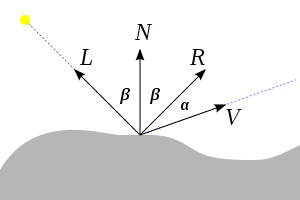
\includegraphics[width=\textwidth]{images/phong-shading-model.png}
    \caption{Phong Shading Model}
\end{figure}

图中的$\alpha$ 很小时,就是高光效果

\begin{math}
    \begin{aligned}
        R = -L + 2(L \cdot N) * N, \\
        I_{spec}=Ks * Il * (dot(V, R))^N_{s}, \\
    \end{aligned}
\end{math}

Ks为镜面反射系数,Ns为高光指数。
Blinn-Phong是基于Phong的修正模型,

\begin{math}
    \begin{aligned}
        H = \frac{L + V}{|L + V|}, \\
        I_{spec} = Ks * Il * (dot(N, H))^N_{s}
    \end{aligned}
\end{math}

H是入射光线方向L与视线方向V的中间向量,称之为半角向量。相比两者,前者更真实,后者高光更柔和,且计算速度较快,
实际中应用更广,OpenGL和DirectX渲染管线中是默认渲染模型。


\subsubsection{全局光照方程}

局部光照模型只考虑光对物体的照明,忽略了物体间的相互影响,其一般公式可以表示为

\begin{math}
    I = I_{abmient} + \sum_{i}^{N}I_{light}\frac{1}{k_{c}+k_{l} \cdot d_{i} + k_{q} \cdot d_{i}^2}
    \left[ k_{d}(N \cdot L) + k_{s}(R \cdot V)^n \right]
\end{math}

每个光源对物体的影响主要包括漫反射和镜面反射两部分,局部照明的阴影算法需要单独考虑。
\newline
全局照明考虑更全面,它自带阴影效果。它主要有两种算法:
\begin{itemize}
    \item {光线追踪法, 关注于镜面反射光,可严格追踪反射光线的方向,实际中采用逆向追踪法,减少计算量}
    \item {辐射度法, 关注于漫反射光,}
\end{itemize}
基本模型是 
\newline

\begin{math}
    \begin{aligned}
        I_r = I_{ia}R_{a} + \sum_{l}I_{il}(N \cdot L_{l})d \omega_{il}(sR_{s} + dR_{d})
    \end{aligned}
\end{math}

其中的环境光和漫反射分量不依赖于观察者的位置View's Position。假设表面是由微面元组成microfacet,其镜面分量为:
\newline

\begin{math}
    \begin{aligned}
        R_s = \frac{F}{\pi} \frac{DG}{\pi (N \cdot L)(N \cdot V)}
    \end{aligned}
\end{math}

为更加丰富,引入了几何项G,Fresnel项F,粗糙度项D。
\newline

\textbf{粗糙度项D},代表了可以有效反射光的那一部分微面元所占的比例,有多种分别函数。
高斯分布模型
\newline

\begin{math}
    \begin{aligned}
        D = ce^{-(\alpha / m)^2}
    \end{aligned}
\end{math}

Bechmann分布函数
\newline

\begin{math}
    \begin{aligned}
        D = \frac{1}{m^2cos^4(\theta)}e^-(tan\alpha / m)^2
    \end{aligned}
\end{math}

\textbf{几何项G},几何衰减项,表现了微小面元之间的互相遮挡shadowing and masking所造成的影响。
\newline

\begin{math}
    \begin{aligned}
        G = \left\{
            1, \frac{2(N \cdot H)(N \cdot V)}{(V \cdot H)}, \frac{2(N \cdot H)(N \cdot L)}{(V \cdot H)} 
        \right\}
    \end{aligned}
\end{math}

\textbf{Fresnel项F},描述了在每一个微面元上光是如何反射,与入射角和波长相关。
\newline

\begin{math}
    \begin{aligned}
        c = cos(\theta) = V \cdot H \\
        g^2 = n^2 + c^2 - 1 \\
    F = \frac{1(g-c)^2}{2(g+c)^2} \left\{ 1+\frac{[c(g+c)-1]^2}{[c(g-c)+1]^2} \right\}
    \end{aligned}
\end{math}


\subsubsection{光照类型}
目前处理光照的思路分两大类,分别是
\begin{itemize}
    \item {逐顶点光照,在每个顶点计算光照,在渲染图元内部进行插值,光照模型中的非线性关系会产生问题}
    \item {逐像素光照,Phong着色,在fragment对顶点法线进行插值}
\end{itemize}

\subsection{渲染类型}

首先从目的出发,真实感渲染与非真实感渲染NPR。

\subsubsection{Photorealistic Rendering}

真实感图形技术包括消隐技术,光照模型,明暗处理和纹理,阴影生成等

\begin{itemize}
    \item {局部光照,仅处理光源直接照射物体表面的光照模型,与光栅化渲染算法相适应的,一次只考虑
    一个像素的光照强度,逐像素的光照计算,不能得到其他像素的光照影响值}
    \begin{itemize}
        \item {Lambert漫反射模型,不能很好处理镜面与高光}
        \item {Gourand}
        \item {Phong,支持高光与镜面}
        \item {Blinn-Phong,速度快,目前商业普遍使用}
        \item {Cook-Torrance,以双向反射的基础上}
    \end{itemize}
    \item {全局光照,基于光学物理原理,光照强度的计算依赖于光能在现实世界中的传播,考虑光线与整个场景中
    各物体表面以及物体表面之间的相互影响,包括多次反射、透射、散射等,成熟应用在离线渲染中}
    \begin{itemize}
        \item {光线跟踪,模拟光从光源出发经过若干次反射、折射达到摄像机的过程,由于只有最终到达摄像机的光线
        才对生成图像有贡献,实现中是以摄像机逆向发出光线,以寻求达到光源的路径。}
        \begin{itemize}
            \item {路径跟踪Path Tracing}
            \item {递归光线追踪Whitte-type}
            \item {分布式光线追踪Distrubution}
            \item {双向路径追踪Bidirectional Path}
            \item {Metropolis}
        \end{itemize}
        \item {辐射度算法,是一种物体空间的算法,用于解离散点或环境中表面曲面面片的光强度问题,而不是解图像平面
        投影的像素问题}
        \item {光子映射,改善漫反射辉映,焦散等全局光照效果,还无法应用在实时渲染中}
    \end{itemize}
\end{itemize}

\subsubsection{Non-Photorealistic Rendering}
对于某些场景,不需要真实感,需要一些艺术化的表现
钢笔素描的生成,
中国国画与书法的生成。
\newline
\textbf{Artistic Shading},艺术渲染,模拟人简画的素描之类的,是一种根据轮廓来来抽象效果。

\subsubsection{基于图像的渲染}
Image Based Rendering,IBR。完全摒弃传统的先建模,然后确定光源的渲染方法,它直接从一系列已知的图像中生成未知
视角的图像,适用于野外极其复杂场景的生成和漫游。